\documentclass[tikz]{standalone}
\usetikzlibrary{shapes, arrows.meta}

\tikzset{
    vertex/.style={circle, draw, fill=blue!20, inner sep=5pt},
    edge/.style={->, thick}
}

\begin{document}
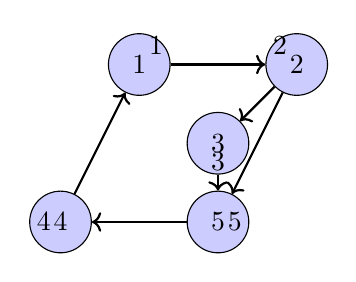
\begin{tikzpicture}[node distance=1cm]
    % Original vertices
    \node[vertex] (v1) at (0,0) {1};
    \node[vertex] (v2) at (2,0) {2};
    \node[vertex] (v4) at (-1,-2) {4};
    \node[vertex] (v5) at (1,-2) {5};
    
    % Edges of the original graph
    \draw[edge] (v1) -- (v2);
    \draw[edge] (v2) -- (v5);
    \draw[edge] (v5) -- (v4);
    \draw[edge] (v4) -- (v1);
    
    % New vertex added
    \node[vertex] (v3) at (1,-1) {3};
    
    % New edges added
    \draw[edge] (v2) -- (v3);
    \draw[edge] (v3) -- (v5);
    
    % Labels for clarity
    \node[above right] at (v1) {1};
    \node[above left] at (v2) {2};
    \node[left] at (v4) {4};
    \node[right] at (v5) {5};
    \node[below] at (v3) {3};
\end{tikzpicture}
\end{document}